<<<<<<<
\newpage
\subsection{Tiefpass}
Die Dimensionierung des Tiefpasses ist von zentraler Bedeutung bei der Rekonstruktion des Nachrichtensignals. Neben der Filtersteilheit und der Restwelligkeit sind Kennwerte wie Ausgangs- und Eingangswiderstand wichtig für die optmale Gestaltung des Tiefpasses.
\subsubsection{Filtercharakteristiken im Vergleich} 
\begin{floatingfigure}[r]{7cm}
	\includegraphics[width=6.5cm]{gfx/simRx/characteristics.png}
	\caption{Filtercharakteristiken}
\label{fig:characteristics}
\end{floatingfigure}
\noindent
Bei aktiven und mehrstufigen Filtertopologien gibt es eine große Auswahl an Fitlercharakteristiken, welche sich durch verschiedene Eigenschaften auszeichnen. Kennwerte für diese Charakteristiken sind Linearphasigkeit, Gruppenlaufzeit, sowie Restwelligkeit im Pass-und Sperrband. In Abbildung \ref{fig:characteristics} sind einige Charakteristiken beispielhaft dargestellt. Für die Rekonstruktion wird eine Butterworth-Charakteristik gewählt, da diese im Passband eine konstante Verstärkung aufweist, sowie keinen Peak kurz vor der Grenzfrequenz hat.\\

\subsubsection{Dimensionierung des Filters}
Zur Dimensionierung des Filters wurde die Designsoftware \textsc{FilterPro} von Texas Instruments verwendet. Als Designparameter wurden neben der Butter\-worth-Charakteristik, eine Verstärkung von 0dB, eine Dämpfung von 60dB je Dekade (Filter 3. Ordnung), Bauteile der E12 Reihe, eine Grenzfrequenz von $f_g=100Hz$ und eine Multiple-Feedback Topologie vorgegeben. Diese Topologie hat im Gegensatz zur Sallen-Key Topologie den Vorteil eines hohen Ausgangswiderstandes. Die Verstärkung von 0dB wird gewählt, da eine Endstufe mit variabler Verstärkung dieser Komponente folgt.
\begin{figure}[H]
	\centering
	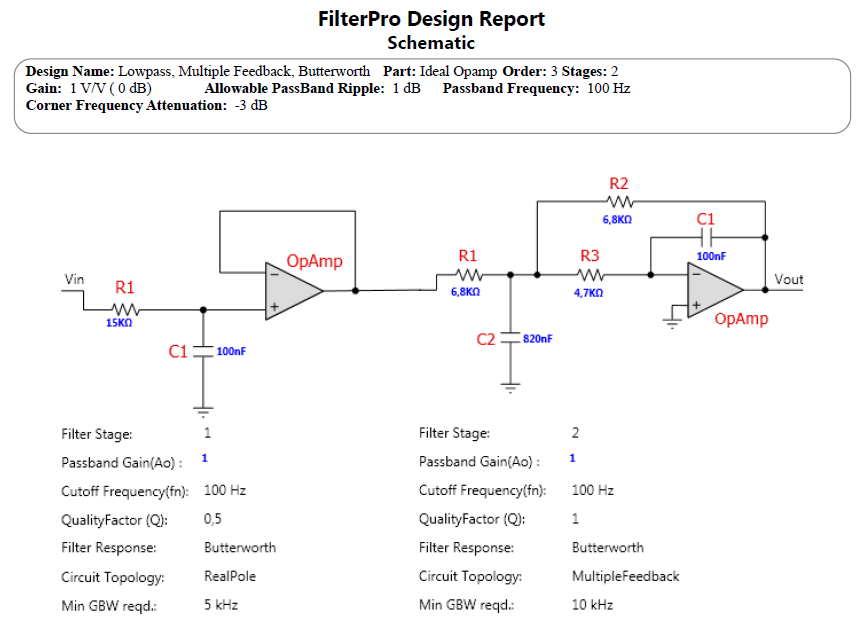
\includegraphics[scale=0.575]{gfx/Butterworth_FilterPro.png}
	\caption{Auszug Design Report}
	\label{fig:design_report}
\end{figure}
\noindent
Der Designreport zeigt die gewünschten Filterparameter. Besonders wichtig an dieser Stelle ist die benötigte Unity-Gain (Gain-Bandwidth-Product), welche sich mit maximal $10kHz$ innerhalb der Spezifikationen vom \textsc{TL074} befinden. Darüber hinaus wurde aufgrund besserer Beschaffbarkeit $C_2$ zu $1\mu F$ gewählt.
\begin{figure}[H]
	\centering
	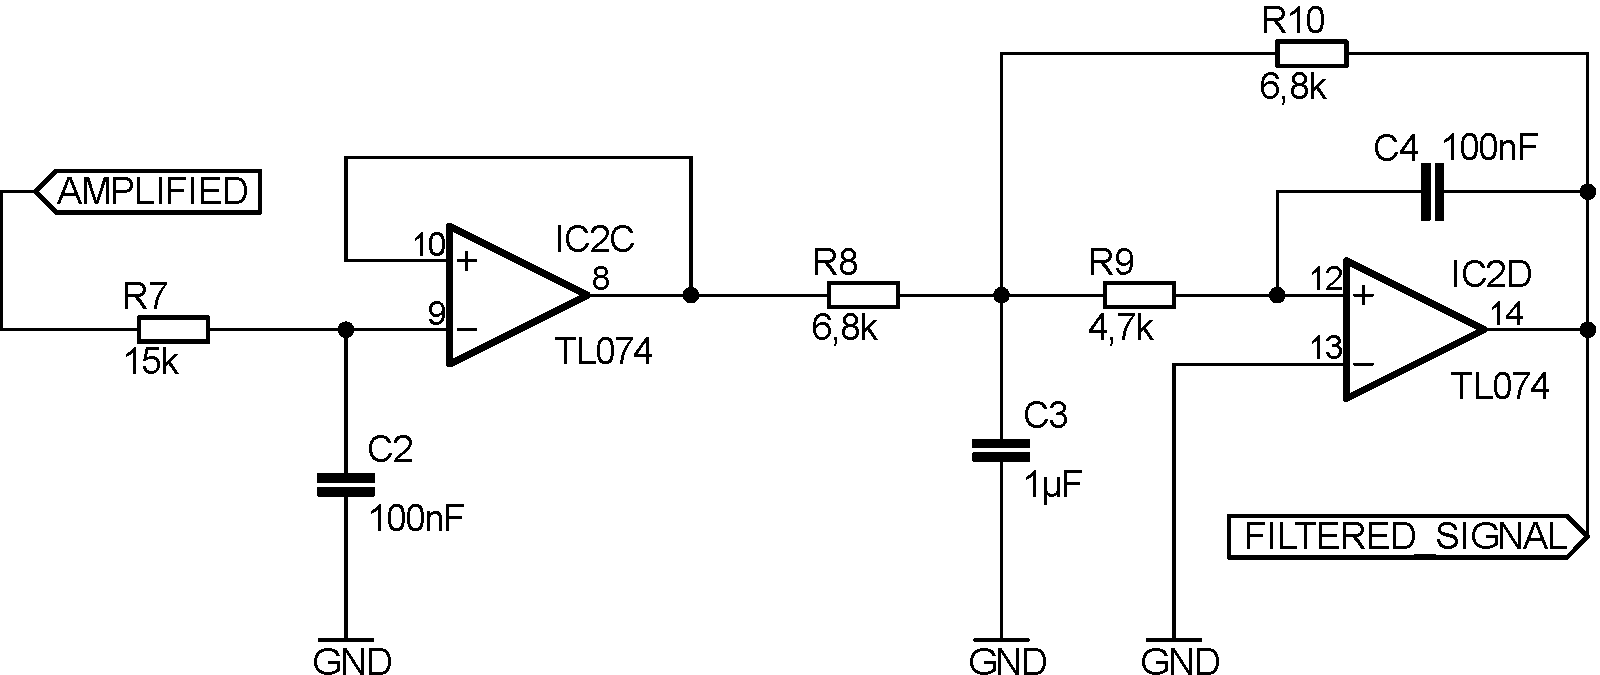
\includegraphics[scale=0.5]{gfx/filter.pdf}
	\caption{Butterworth-Tiefpass}
\end{figure}
\noindent
Der Widerstand $R_7$ und der Kondensator $C_2$ bilden als passiver Tiefpass die erste Filterstufe. Diese ist mit dem linken Operationsverstärker, welcher als Spannungsfolger beschaltet ist von der nachfolgenden zweiten Filterstufe entkoppelt. Mit $R_8$ und $C_3$ folgt ein weiterer passiver Tiefpass. Der letzte Teil des Filters ist ein aktiver Tiefpass, der sich aus dem zweiten Operationsverstärker und den Widerständen $R_9$ ,$R_{10}$, sowie dem Kondensator $C_4$ zusammensetzt.








=======
\newpage
\subsection{Tiefpass}
Die Dimensionierung des Tiefpasses ist von zentraler Bedeutung bei der Rekonstruktion des Nachrichtensignals. Neben der Filtersteilheit und der Restwelligkeit sind Kennwerte wie Ausgangs- und Eingangswiderstand wichtig für die optmale Gestaltung des Tiefpasses.
\subsubsection{Filtercharakteristiken im Vergleich} 
\begin{floatingfigure}[r]{7cm}
	\includegraphics[width=6.5cm]{gfx/characteristics.png}
	\caption{Filtercharakteristiken}
\label{fig:characteristics}
\end{floatingfigure}
\noindent
Bei aktiven und mehrstufigen Filtertopologien gibt es eine große Auswahl an Fitlercharakteristiken, welche sich durch verschiedene Eigenschaften auszeichnen. Kennwerte für diese Charakteristiken sind Linearphasigkeit, Gruppenlaufzeit, sowie Restwelligkeit im Pass-und Sperrband. In Abbildung \ref{fig:characteristics} sind einige Charakteristiken beispielhaft dargestellt. Für die Rekonstruktion wird eine Butterworth-Charakteristik gewählt, da diese im Passband eine konstante Verstärkung aufweist, sowie keinen Peak kurz vor der Grenzfrequenz hat.\\

\subsubsection{Dimensionierung des Filters}
Zur Dimensionierung des Filters wurde die Designsoftware \textsc{FilterPro} von Texas Instruments verwendet. Als Designparameter wurden neben der Butter\-worth-Charakteristik, eine Verstärkung von 0dB, eine Dämpfung von 9dB je Dekade (Filter 3. Ordnung), Bauteile der E12 Reihe, eine Grenzfrequenz von $f_g=100Hz$ und eine Multiple-Feedback Topologie vorgegeben. Diese Topologie hat im Gegensatz zur Sallen-Key Topologie den Vorteil eines hohen Ausgangswiderstandes. Die Verstärkung von 0dB wird gewählt, da eine Endstufe mit variabler Verstärkung dieser Komponente folgt.
\begin{figure}[H]
	\centering
	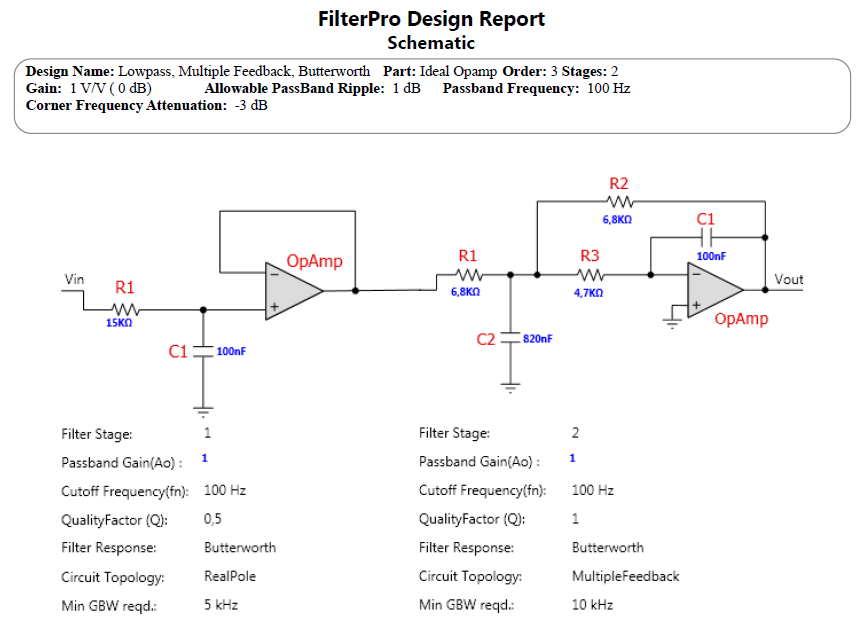
\includegraphics[scale=0.575]{gfx/Butterworth_FilterPro.png}
	\caption{Auszug Design Report}
	\label{fig:design_report}
\end{figure}
\noindent
Der Designreport zeigt die gewünschten Filterparameter. Besonders wichtig an dieser Stelle ist die benötigte Unity-Gain (Gain-Bandwidth-Product), welche sich mit maximal $10kHz$ innerhalb der Spezifikationen vom \textsc{TL074} befinden. Darüber hinaus wurde aufgrund besserer Beschaffbarkeit $C_2$ zu $1\mu F$ gewählt.
\begin{figure}[H]
	\centering
	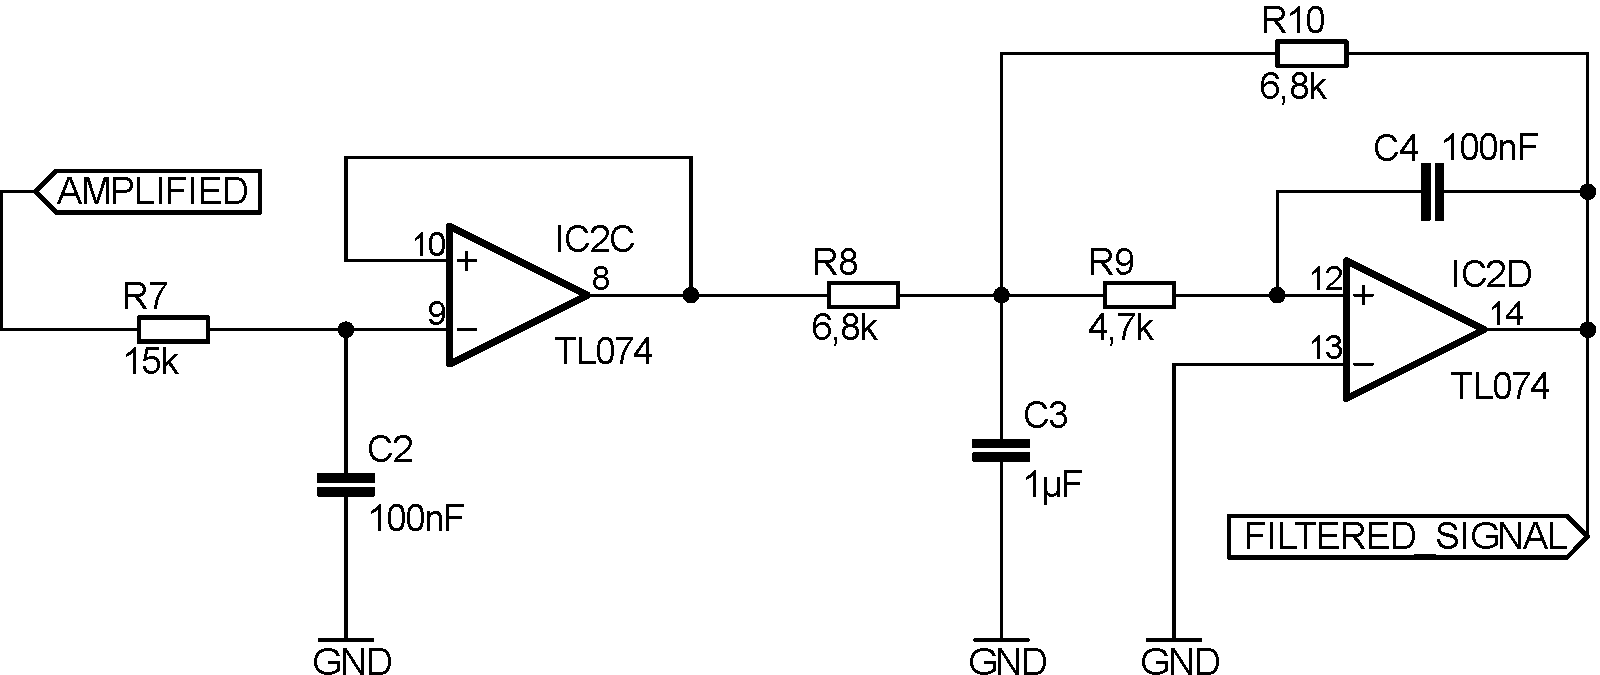
\includegraphics[scale=0.5]{gfx/filter.pdf}
	\caption{Butterworth-Tiefpass}
\end{figure}
\noindent
Der Widerstand $R_7$ und der Kondensator $C_2$ bilden als passiver Tiefpass die erste Filterstufe. Diese ist mit dem linken Operationsverstärker, welcher als Spannungsfolger beschaltet ist von der nachfolgenden zweiten Filterstufe entkoppelt. Mit $R_8$ und $C_3$ folgt ein weiterer passiver Tiefpass. Der letzte Teil des Filters ist ein aktiver Tiefpass, der sich aus dem zweiten Operationsverstärker und den Widerständen $R_9$ ,$R_{10}$, sowie dem Kondensator $C_4$ zusammensetzt.








>>>>>>>